\section{Market \& Industry}
\subsection{Industry definition} 
BottAll will compete in the food and beverage storage container industries. The industry comprises different manufacturers, some that create both lunch boxes and reusable water bottles, and others that make only one of these two type of products. Well-known companies in this market includes Tupperware, Chilly’s, Blue Dopper, Mira and, the established Italian company, 24 Bottles. 

\subsection{Industry size} 
The industry is in the growing phase of its life cycle. Growth is being driven by a lot of factors, but primarily by the growing awareness of environmental pollution and the attention to what we eat (talking about healthy food trend).\\
According to Grand View Research, an American institute specialized in market analysis, the reusable water bottles market in 2018 generated a turnover of 8.1 billion of dollar and it will grow by the 3.5\% each year from today to 2025. \\
The global market for Lunch Boxes from \$2.7 billion in 2017 is anticipated to reach \$5.96 billion by 2024. It is expected to raise by 12\% through 2024 (2018 to 2024). Increasing attention to nutrition for all people will drive the growth of the market in the coming years.
\begin{figure}[H]
\centering
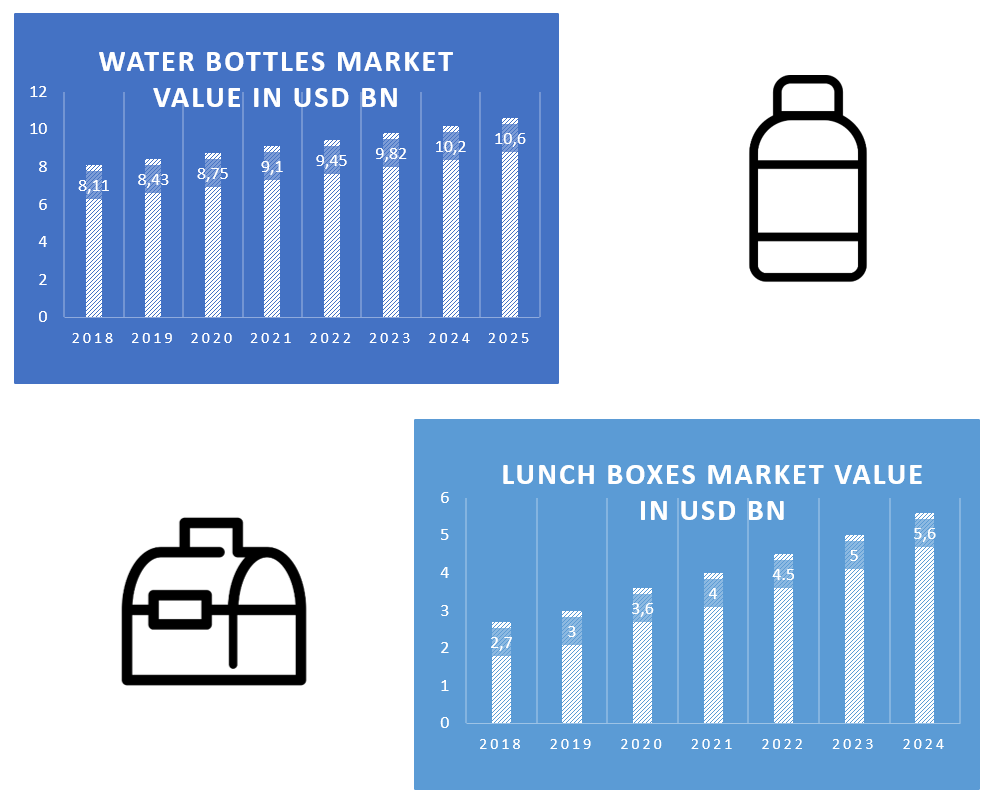
\includegraphics[width=0.7\textwidth]{images/bottle_lunch_market.PNG}
\caption{Water Bottle and Food container market Value}
\end{figure}
There are various environmental and business trends affecting the growth and attractiveness of the food and beverage storage container industry.

\subsection{Trend That Favour the Industry}
\begin{itemize}
\item People are increasingly aware about climate change related to pollution.
\item More attention to nutrition.
\item New governments laws that forbid the usage of plastic and non-reusable plastic plates.
\item More and more people do not have enough time to eat during work and university break.
\end{itemize}

\subsection{Trend working against the Industry}
\begin{itemize}
\item Food delivery service with competitive prices.
\item Supermarkets selling ready-to-eat foods.
\end{itemize}

\subsection{Long term prospects}
The industry is likely to maintain its current trajectory. Obviously, an increasing interest in Eco-friendly life style will help this market to grow but also the interest of people regarding the style of these products is a very important point, more and more people are going to desire an high-end product instead of a cheap and unsightly one.

\subsection{Market Analysis}
According to the data found in~\cite{dati_pranzo} we were able to identify our market segment. The market of our purpose takes in account students and workers with an age between 18 and 55 years old. Half of the interviewed people stated to eat at the office or at university 2/3 times per week. However, the 65\% of workers and 78\% of students that decide to stay out during the break to have lunch, eat home cooked meals. In this final data, we found our market of interest focusing on people that want a high-end Eco-friendly product that allows them to enjoy a hot meal and a good beverage.
Based on the above information it was possible to segment the market looking at our primary market.

\begin{figure}[H]
\centering
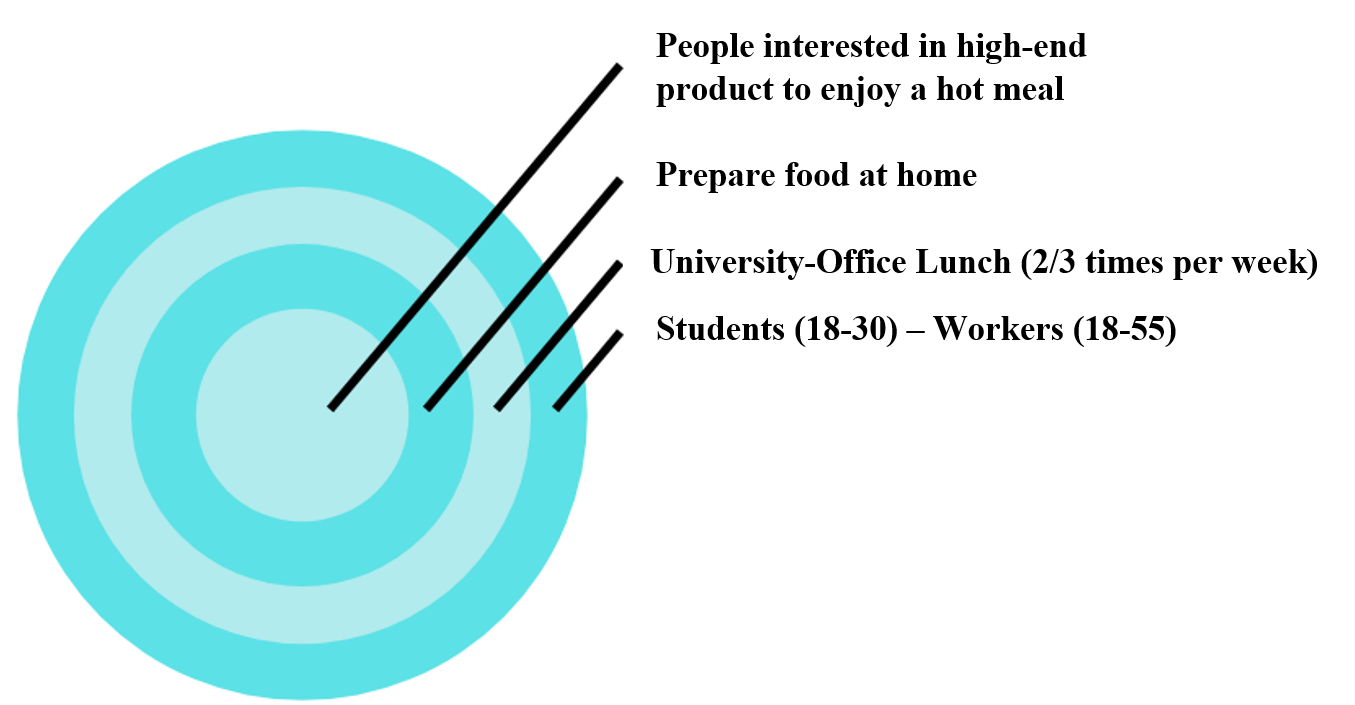
\includegraphics[width=0.7\textwidth]{images/market_chart.PNG}
\caption{Market analysis Chart}
\end{figure}

\subsection{Competitor Analysis}
The best solution to the problem outlined above is to create a stylish food and beverage storage container to enjoy the lunch break. For the purposes of this business plan we delineated some of the most important direct competitors and we spent a few words for the indirect ones.

\subsubsection{Direct competitors}
Currently, there are several competitors that use different shapes, materials and styles to create their products but no one have a 2in1 solution to store both food and drink and no one use electronics inside the storage container to warm up the food. For space reasons, in this business we will focus only on the major players of this industry.
\begin{itemize}
\item \textbf{Mira}, \textbf{S’Well} and \textbf{Chilly’s} have a similar product in their catalogue. They produce both water and food storage containers using BPA free material and insulated stainless steel which allows food and beverage to stay hot or cold for hours. They also offer the possibility to choose the same product in different sizes and colours to meet all customers needs.
\item \textbf{24 Bottles} is the most important Italian brand in this type of industry. At the moment, they are focusing on developing different bottles for drink, using only BPA free materials. They offer both insulated stainless steel products and not insulated bottles. The customer can choose the same product with different colours and particular design.
\item \textbf{Tupperware} is a well-known American multinational company focused on kitchen and household products. In the catalogue they offer some food containers and some bottles but they are only made in reusable plastic.
\item \textbf{Golchi} is a start-up that presented their product through a Kickstarter campaign. The product is a reusable water bottle with a 2in1 solution which allows the customers to bring two drinks simultaneously in any combination of hot and cold.
\end{itemize}

\subsubsection{Indirect competitors}

Indirect competitors are delivery services, supermarkets selling ready-to-eat dishes including some bars and restaurants with competitive lunch menu formulas (in terms of price).
A recap table was made to highlight the different features.

\begin{table}[H]
\centering
\caption{Competitors Comparition}
\begin{tabular}{cccccc}
\toprule
 & \textbf{Food storage} & \textbf{Drink storage} & \textbf{BPA free} & \textbf{2in1} & \textbf{Internal heater}\\
\toprule
\textbf{Mira} & \textcolor{ForestGreen}{YES} & \textcolor{ForestGreen}{YES} & \textcolor{ForestGreen}{YES} & \textcolor{red}{NO} & \textcolor{red}{NO}\\
\hline
\textbf{S’well} & \textcolor{ForestGreen}{YES} & \textcolor{ForestGreen}{YES} & \textcolor{ForestGreen}{YES} & \textcolor{red}{NO} & \textcolor{red}{NO}\\
\hline
\textbf{Chilly’s} & \textcolor{ForestGreen}{YES} & \textcolor{ForestGreen}{YES} & \textcolor{ForestGreen}{YES} & \textcolor{red}{NO} & \textcolor{red}{NO}\\
\hline
\textbf{24 Bottles} & \textcolor{red}{NO} & \textcolor{ForestGreen}{YES} & \textcolor{ForestGreen}{YES} & \textcolor{red}{NO} & \textcolor{red}{NO}\\
\hline
\textbf{Tupperware} & \textcolor{ForestGreen}{YES} & \textcolor{ForestGreen}{YES} & \textcolor{red}{NO} & \textcolor{red}{NO} & \textcolor{red}{NO}\\
\hline
\textbf{Golchi} & \textcolor{red}{NO} & \textcolor{ForestGreen}{YES} & \textcolor{ForestGreen}{YES} & \textcolor{ForestGreen}{YES} & \textcolor{red}{NO}\\
\hline
\textbf{BottAll} & \textcolor{ForestGreen}{YES} & \textcolor{ForestGreen}{YES} & \textcolor{ForestGreen}{YES} & \textcolor{ForestGreen}{YES} & \textcolor{ForestGreen}{YES}\\

\bottomrule
\end{tabular}
\end{table}